%----------------------------------------------------------------------------
% Start
%----------------------------------------------------------------------------

\documentclass{article}

\usepackage{enumerate}
\usepackage{graphicx} % Required for the inclusion of images 
\usepackage{tocloft}
\usepackage{url} % References include URLs
\usepackage{mathtools} % Math stuff
\usepackage[export]{adjustbox}
\usepackage{hyperref} % Makes links actually work!=
\usepackage{geometry}

\renewcommand{\cftsecleader}{\cftdotfill{\cftdotsep}} 
\renewcommand{\labelenumi}{\theenumi.}
\renewcommand{\labelenumii}{\alph{enumii}.}

\geometry {a4paper, left = 30mm}
\renewcommand{\baselinestretch}{1.5}
\setlength{\parskip}{1em}
\setlength\parindent{0pt} % Removes all indentation from paragraphs


%----------------------------------------------------------------------------
% Document Information
%----------------------------------------------------------------------------

\begin{document}

\title{COSC450: k-means Segmentation}
\author{Ashley Manson}
\date{\today}

\begin{titlepage}
\clearpage
\maketitle
\thispagestyle{empty} % Remove page number from title page

\begin{center}

\vspace*{1\baselineskip} % Skip a line

Department of Computer Science\\
University of Otago

\end{center}

\end{titlepage}

%----------------------------------------------------------------------------
% My Code
%----------------------------------------------------------------------------

\section{Program and Code}
The code is compiled with the included Makefile, if the setPath.sh has run
sucessfully on the lab machines.\\ 

The program takes 7 command line arguments in this order:
\begin{enumerate}
\item The input image to perform the segmentation on.
\item An output image to save the result.
\item k for the number of clusters.
\item Cluster type, which is a number between 0 and 2.
  \begin{enumerate}
  \item 0 is for random selection.
  \item 1 is for random clustering.
  \item 2 is for k-means++.
  \end{enumerate}
\item Distance type is a number between 0 and 1.
  \begin{enumerate}
  \item 0 is for comparing RGB values.
  \item 1 is for comparing HSV values.
  \end{enumerate}
\item Termination type is a number between 0 and 2.
  \begin{enumerate}
  \item 0 is for giving the maximum iterations before terminating.
  \item 1 is for terminating once the clusters have stopped making changes. A
    value at the top of the file CLUSTER\_MIN\_CHANGE can augment this.
  \item 2 is for terminating once the labels have stopped making changes. A value
    at the top of the file LABEL\_MIN\_CHANGE can augment this.
  \end{enumerate}
\item Max iterations is for giving a maximum number of iterations before the
  program will terminate. Will be used if 0 is given for the end type.
\end{enumerate}

Once the first image has been displayed, a key press will begin the k-means
segmentation. Output will be printed to stdout of the progress so far. Once the
k-means algorithm completes, the segmented image will be displayed. Sometimes it
displays behind the original, so moving the original image will reveal the
segmented image. Another key press once the segmented image is displayed will
close both windows. The segmented image will be saved to the given command line
argument for viewing later.

%----------------------------------------------------------------------------
% Implementation
%----------------------------------------------------------------------------

\section{Implementation}

\subsection{Initialisation Methods}
I have implemented the three initialisation methods that were proposed in the
Assignment 2 specifications; random selection, random clustering, and k-means++.

\subsubsection{Random Selection}
This method of initialisation is the fastest. For each k cluster point, it will
get a random x and y coordinate that corresponds to a pixel in the image. This
is then added to a vector of Vec3b for computation later.

\subsubsection{Random Clustering}
This initialisation method is slower than selection as it goes through all the
pixels in the image. For each pixel in the image, it is assigned a random k
cluster. Once all pixels from the image have been assigned a k cluster, it goes
through each cluster, calculating the average colour across all the pixels. Once
the average has been calculated, the colour average is added to the clusters
vector for computation later.

\subsubsection{k-Means++}
This method of initialisation takes the longest due to the random distribution
that contributes to the selection of clusters. The first cluster is selected at
random from the image. This serves as the first cluster point. The first loop
then goes over the rest of the clusters that need to be selected. The first
inner loop then goes over the image calculating the distances from the selected
cluster, storing the result in its corresponding index in a vector and adding to
a count. The second inner loop then goes on until another cluster is added to
the cluster vector. Here there is a chance for one of the distances in the
vector to be selected based on a random distribution of all distances
calculated. Once a new k cluster has been found, it is added to the clusters
vector, and this loop exits. All of this is repeated until all k clusters are
found.

\subsection{Distance Metrics}
I have implemented two different ways of calculating the distance of two pixels,
one being the raw RGB values, and the second being the HSV of a pixel, ignoring
the value. For each pixel in the image, I go through and calculate the distance
from it and each of the k cluster points. If the distance is less than the
previous distance, that pixel label gets updated and it gets a new minimum
distance set for it. For RGB, I simply calculate the difference between the
corresponding RGB values. For HSV I scale the hue by dividing by 180 and than
multiply by 256. The reason for this is due to OpenCV storing its hue value
between 0 and 179. The scale ensures that the distance calculations are
correct. When calculating the distance I ignore the value from HSV.

\subsection{Termination Conditions}
I have implemented three different ways for the k-means program to terminate.
It can be passed in a parameter to set the maximum number of iterations that the
program will run for. It can be set to check the differences in cluster
changes. It can be set to check how many labels are changing between iterations.

\subsubsection{Maximum Iterations}
The program can be set to run for a set number of iterations, no matter if it
has stabilized or still has yet to stabilize.

\subsubsection{Cluster Changes}
The program can be set to check for changes in cluster points. With every
iteration, the difference between cluster changes is calculated, and if it is
less than a prespecified minimum change, then the algorithm will terminate.

\subsubsection{Label Changes}
The program can be set to check for changes in labels for each pixel. With every
iteration, the number of changed labels is summed up, and if it is less than a
prespecified minimum change, then the program will terminate.

%---------------------------------------------------------------------------
% Experiments
%---------------------------------------------------------------------------

\section{Experiments}

I have experimented with Random Selection, Random Clustering and k-Means++, as
well as testing each initialisation method with both RGB and HSV. I have ran
each with k clusters of 4, 6, and 8. The termination case was the change of
clusters. I have taken the average of each to find out which is fastest to
segment the image. In the following charts, RS means random selection, RC means
random clustering, and KM means k-means++. The error bars on the charts are of
the standar deviation or error for each average.

\subsection{Average Iterations}

\subsubsection{mms.jpg}

\begin{figure}[ht]
\begin{center}
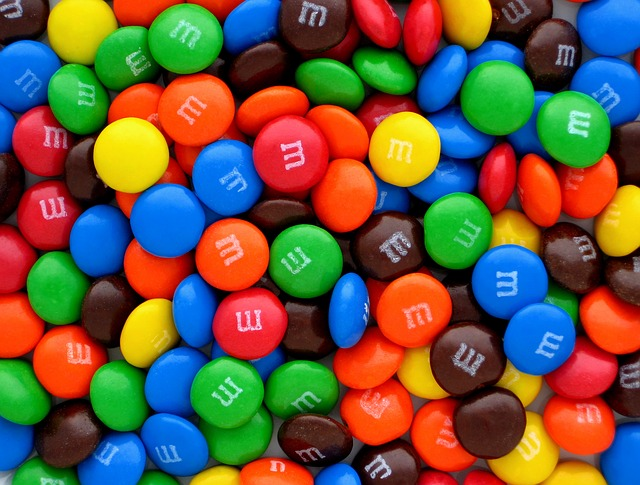
\includegraphics[width=0.35\textwidth]{images/mms}
\caption{Image used for testing mms.jpg.}
\label{fig:mmsTest}
\end{center}
\end{figure}

\begin{figure}[ht]
\begin{center}
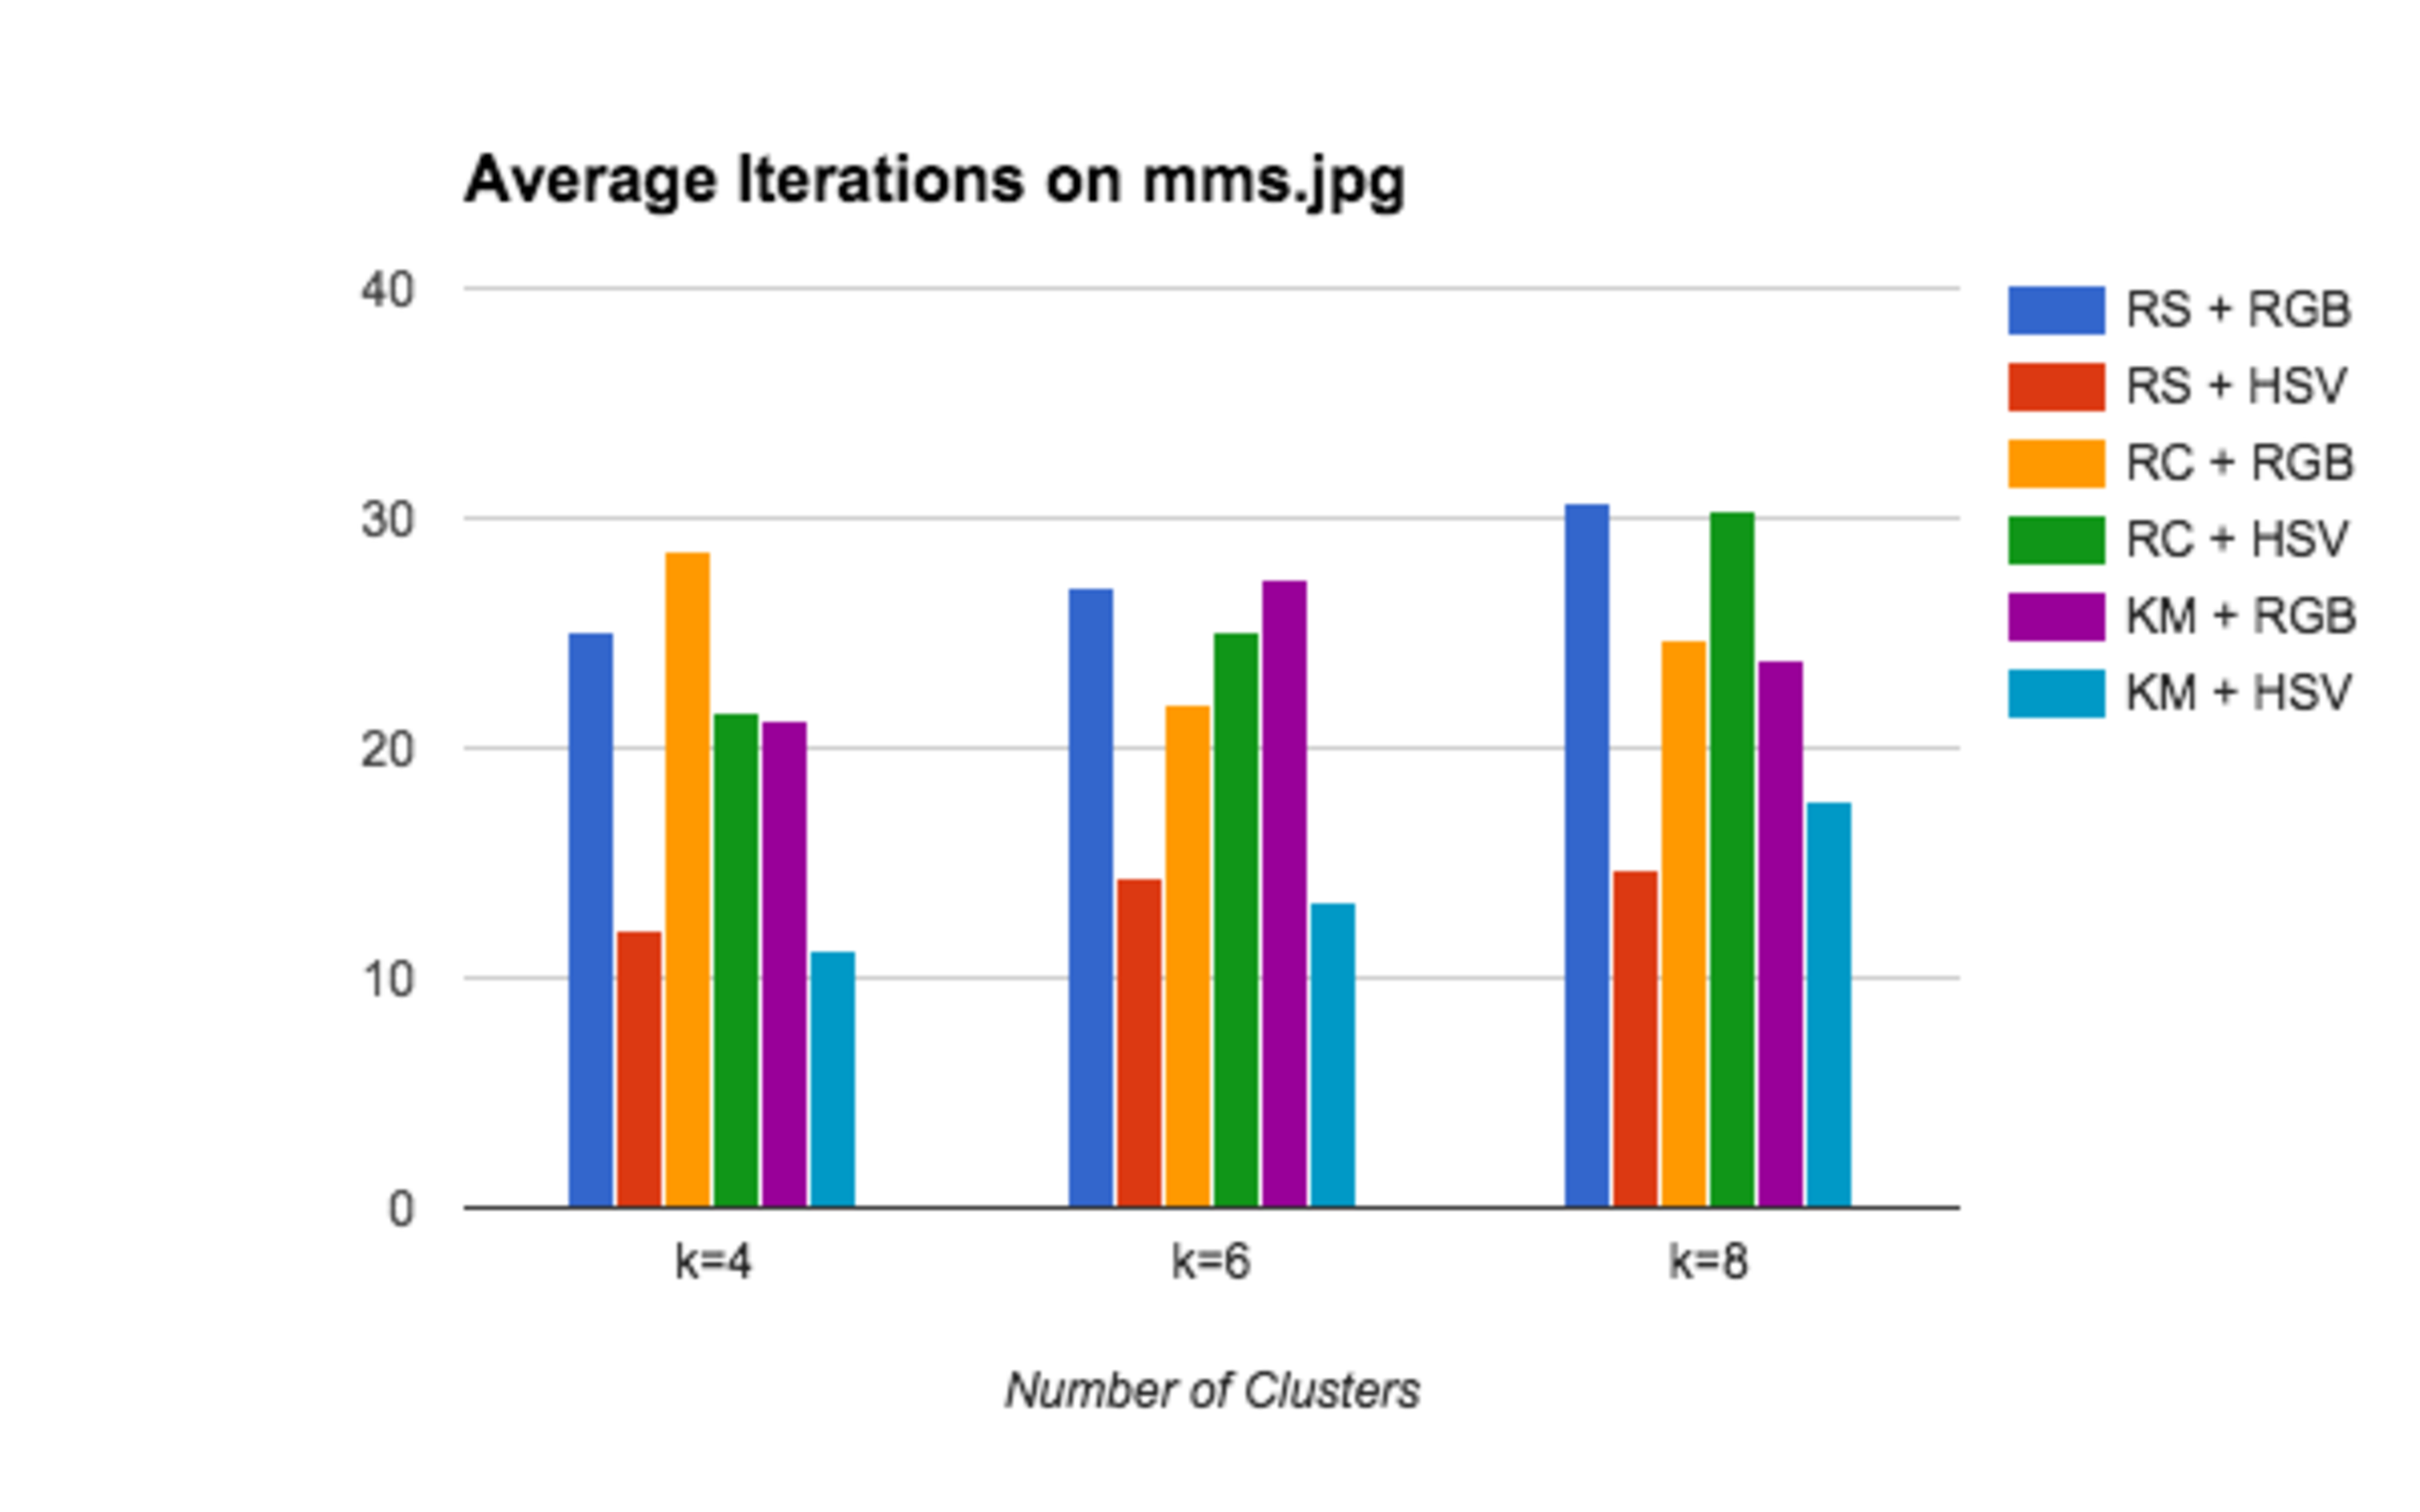
\includegraphics[width=1\textwidth]{images/mmsChart}
\caption{Average iterations on mms.jpg.}
\label{fig:mmsChart}
\end{center}
\end{figure}

Figure \ref{fig:mmsChart} shows that HSV in combination with Random Selection or
k-Means++ performs better than the other distance metrics and initialisation
method combination. Probably due to there being a wider range of colour in this
image for the initialisation methods to select. I believe that the reasont he
clustering falls short is there is too much colour for it to average over, so it
takes longer for it to stabilize the clusters.

\subsubsection{lena.png}

\begin{figure}[ht]
\begin{center}
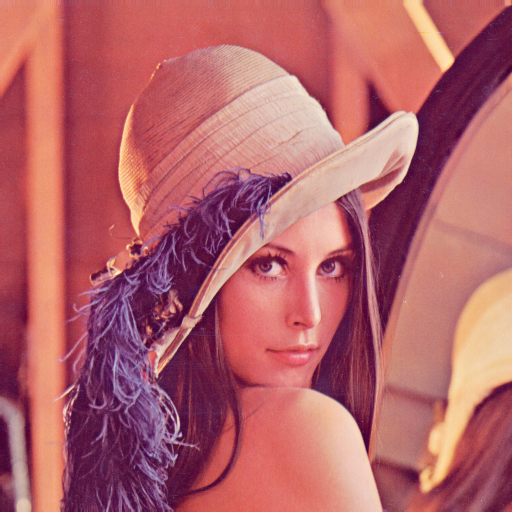
\includegraphics[width=0.35\textwidth]{images/lena}
\caption{Image used for testing lena.png.}
\label{fig:lenaTest}
\end{center}
\end{figure}

\begin{figure}[ht]
\begin{center}
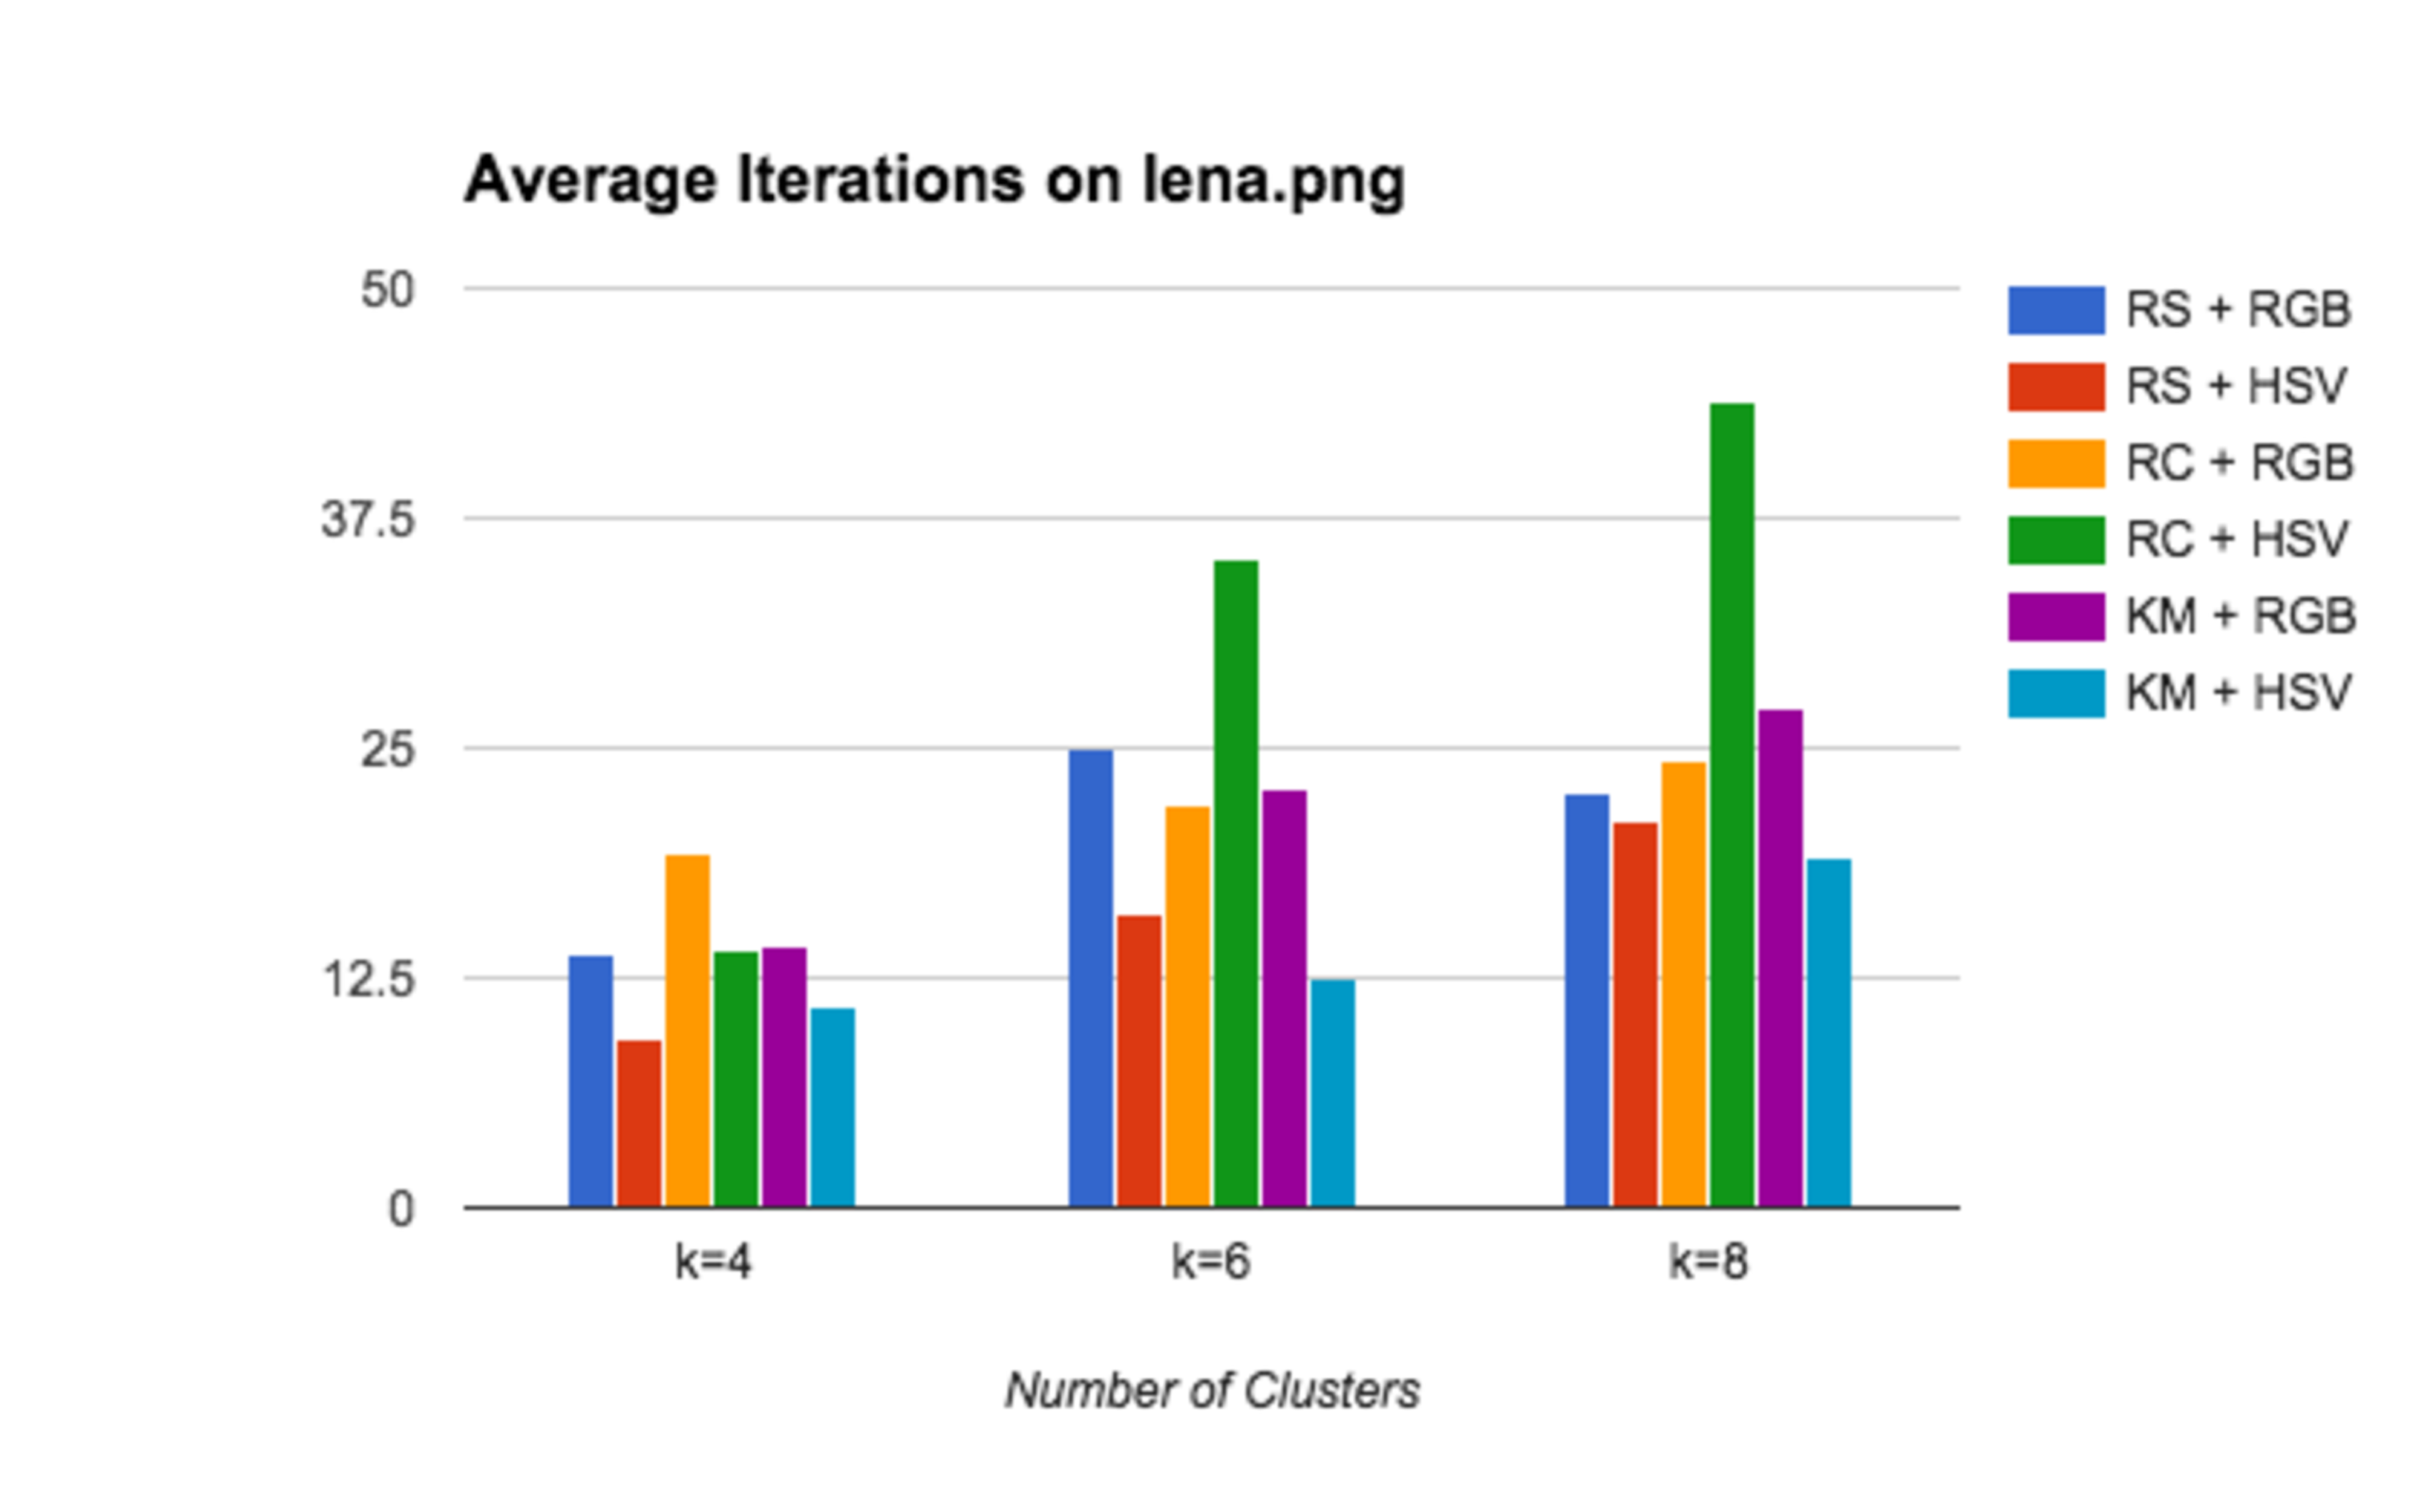
\includegraphics[width=1\textwidth]{images/lenaChart}
\caption{Average iterations on lena.png.}
\label{fig:lenaChart}
\end{center}
\end{figure}

Figure \ref{fig:lenaChart} shows that when k is set to 4, all the combinations
seem to perform around the same level. Moving onto a higher k value however,
random clustering and HSV start to take longer than the rest to
stabilize. k-Means++ with HSV outperform the rest. I believe that this is due to
k-means++ initialising more unique clusters from the image, which allows for the
clusters to stabilize faster.

\subsubsection{penguin.jpeg}

\begin{figure}[ht]
\begin{center}
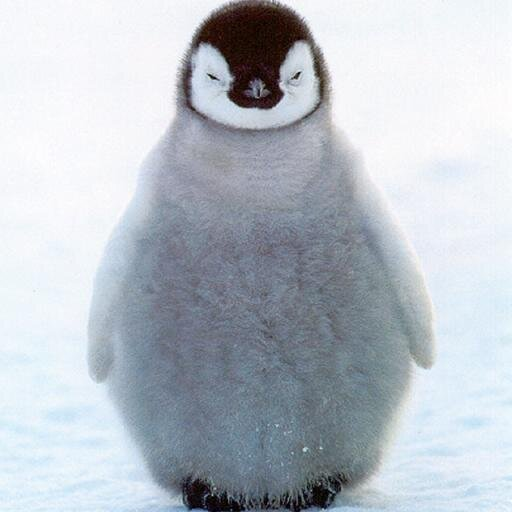
\includegraphics[width=0.35\textwidth]{images/penguin}
\caption{Image used for testing penguin.jpeg.}
\label{fig:penguinTest}
\end{center}
\end{figure}

\begin{figure}[ht]
\begin{center}
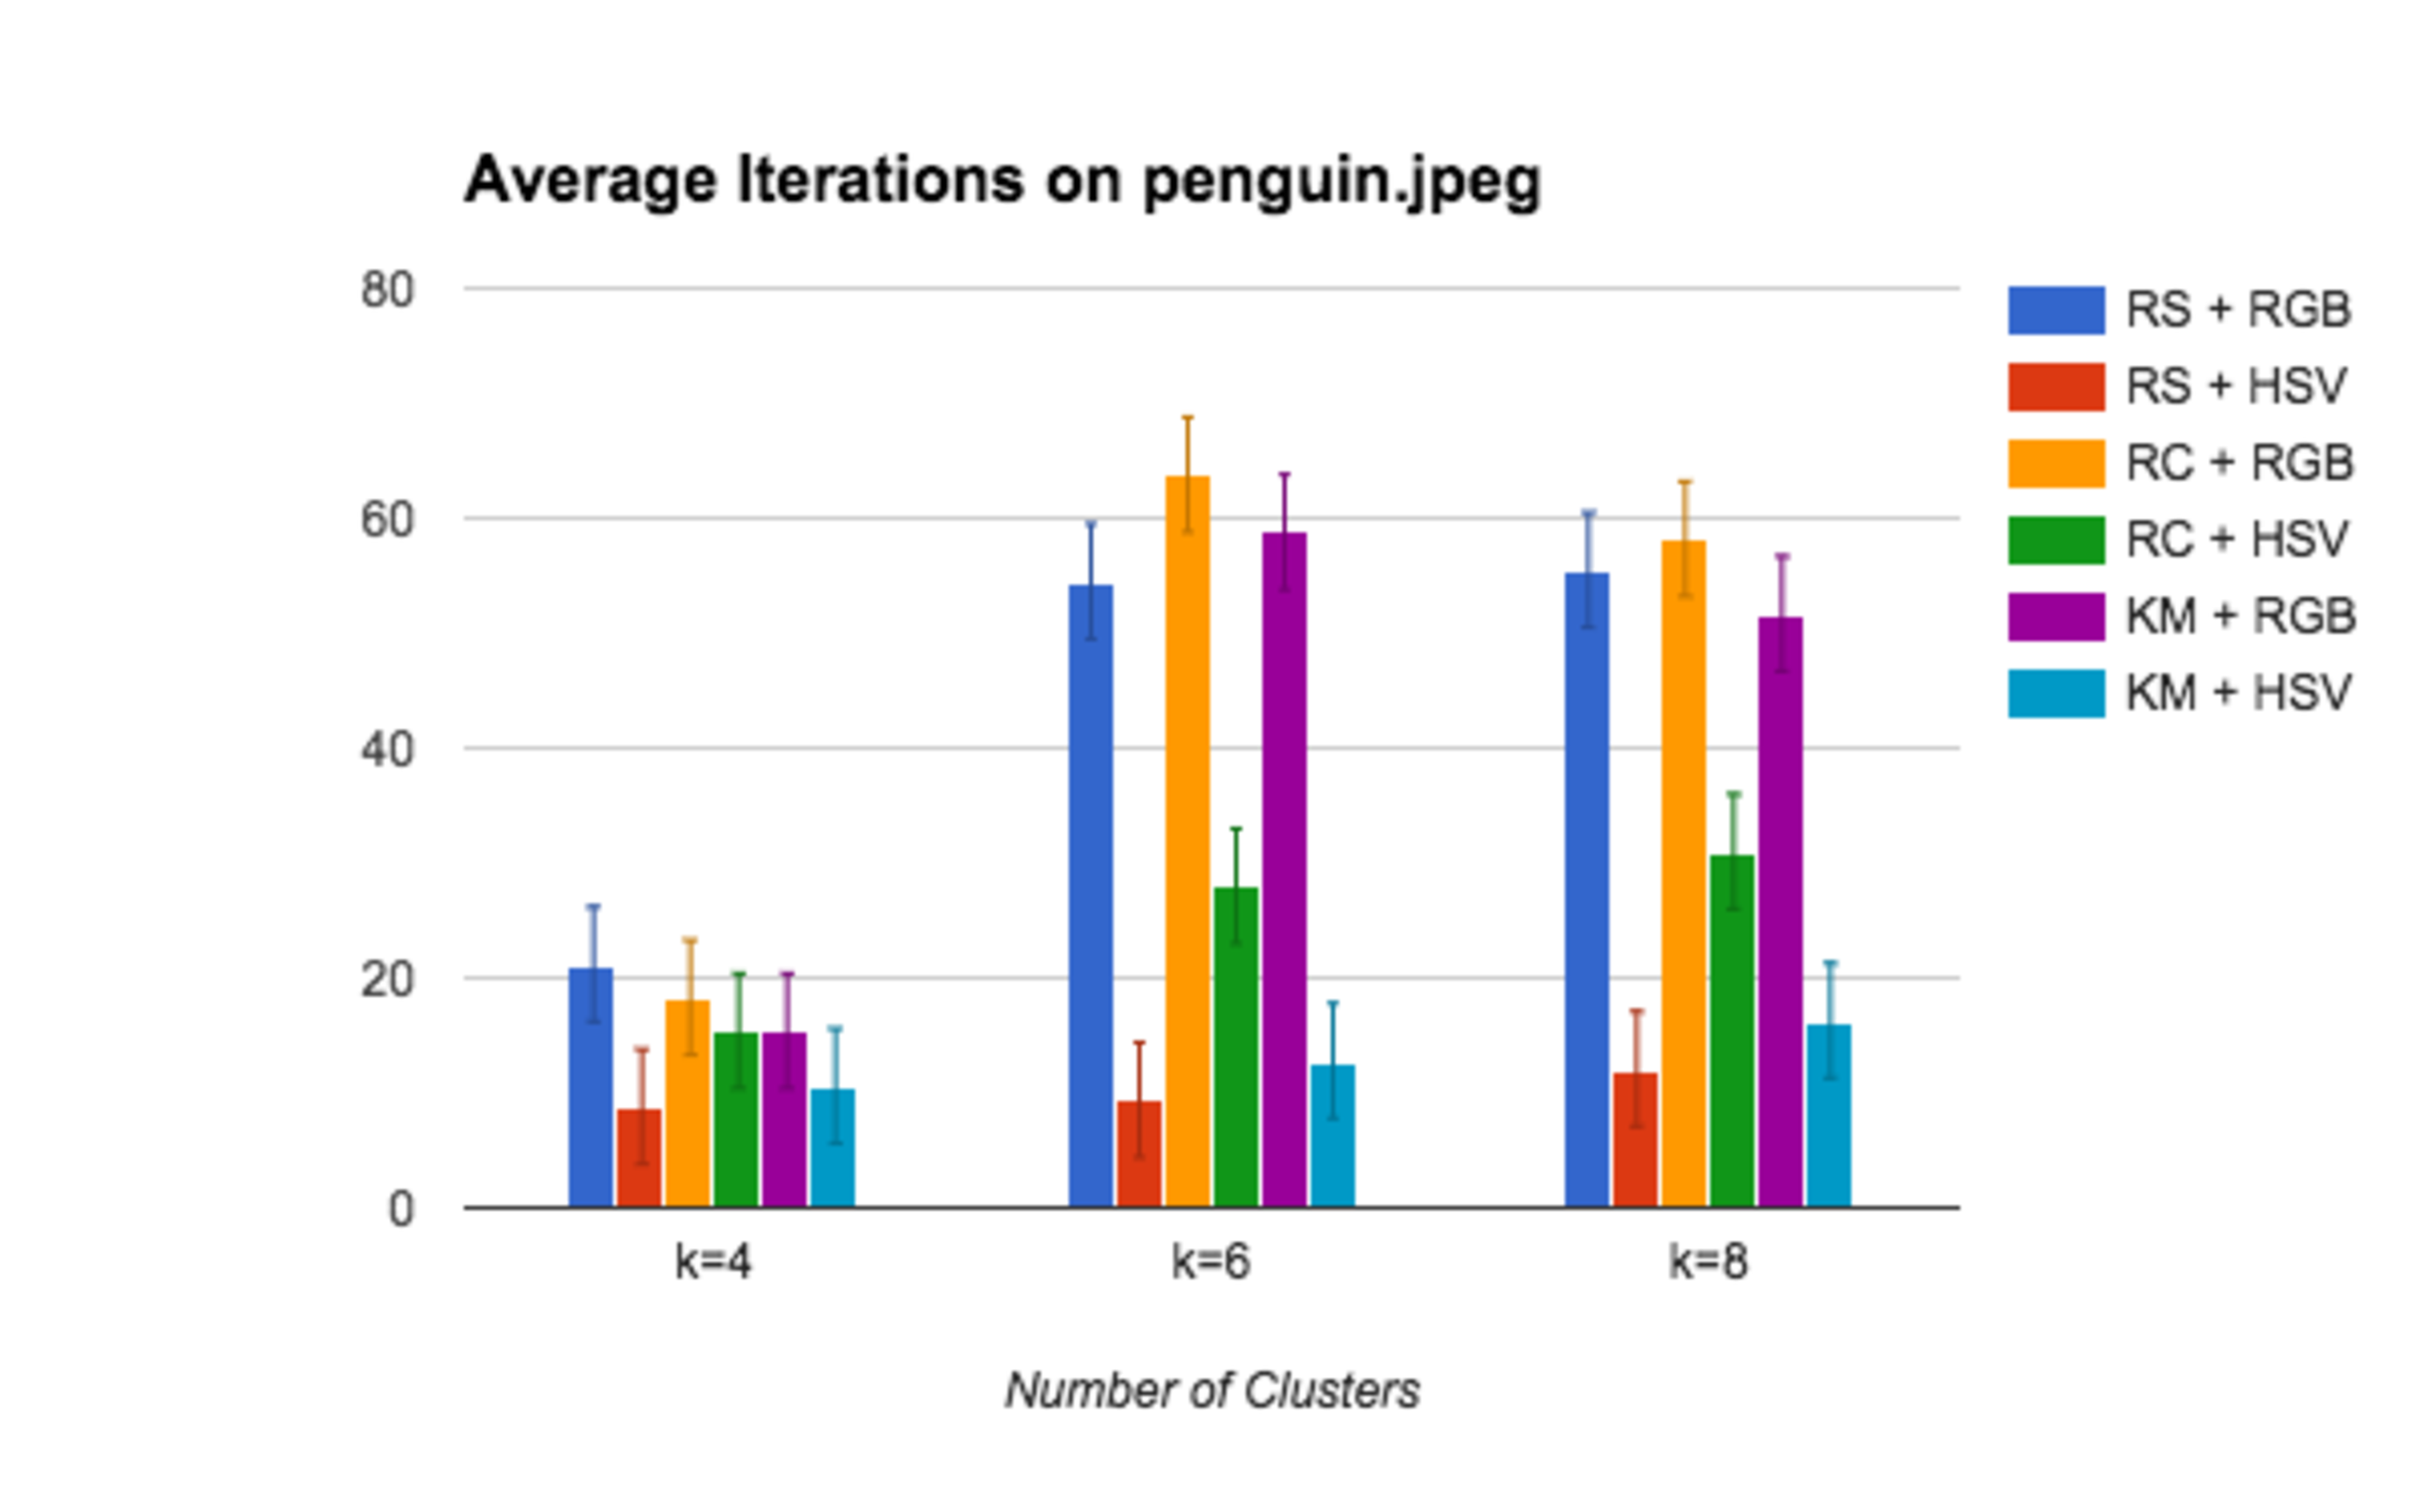
\includegraphics[width=1\textwidth]{images/penguinChart}
\caption{Average iterations on penguin.jpeg.}
\label{fig:penguinChart}
\end{center}
\end{figure}

With Figure \ref{fig:penguinChart} when k is set to 4, all combinations seem to
perform around the same. When k is increased, all RGB combinations perform
horribly. I believe this is caused due to all the clusters trying to stabilise
but all the white in the image is causing this to fail. Due to HSV ignoring
colour and only focusing on hue and saturation, it outperforms the RGB version
in regards to timing.

\subsection{RGB vs HSV}
I have taken a look at the resulting images from RGB and HSV distance metrics. I
have used k-Means++ with the change in clusters as the termination case. I am
looking for which distance metrics segments the image in the best possible way.

\subsubsection{Bear k = 8}

\begin{figure}[ht]
\begin{center}
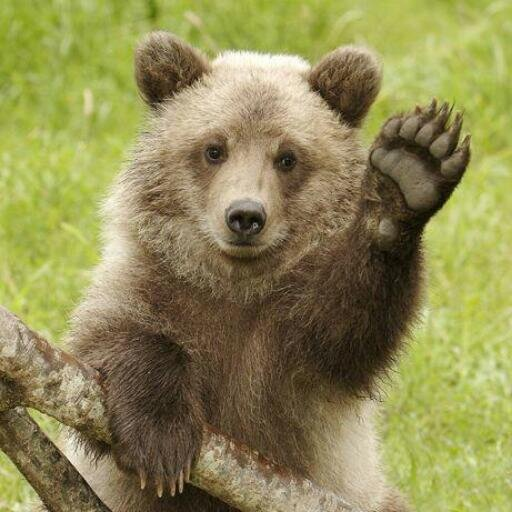
\includegraphics[width=0.3\textwidth]{images/bear}
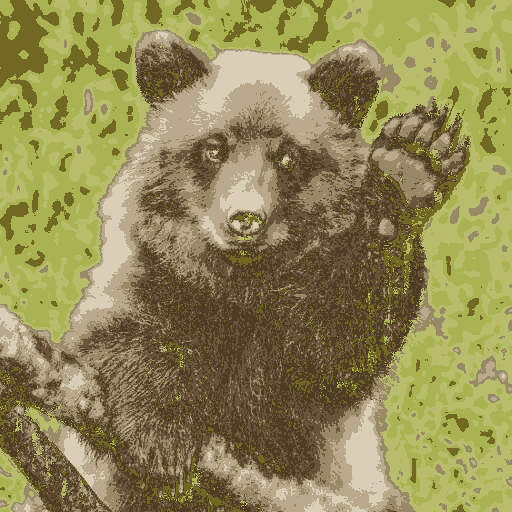
\includegraphics[width=0.3\textwidth]{images/hsv_8_bear}
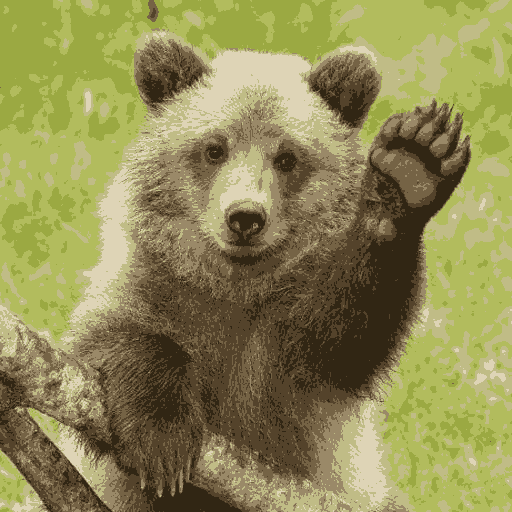
\includegraphics[width=0.3\textwidth]{images/rgb_8_bear}
\caption{Bear Original, HSV and RGB.}
\label{fig:bear}
\end{center}
\end{figure}

For Figure \ref{fig:bear} I choose to have k as 8 for this, as HSV failed to
properly segment the image with any k lower than that. However in this example,
RGB still segments the image better than the HSV version. RGB finds a lot of the
colour from the bear, and does not blend it with the green background, unlike
the HSV version. The HSV version seems to be picking up on incorrect value on
the bear, and clusters some of it with the green background. This could be
caused by the bears brown fur having a similar hue/saturation as the gree
background on the top left of the image. The RGB version is better segmented as
it is more easily distinguished from the rest of the image.

\subsubsection{Kitten k = 5}

\begin{figure}[ht]
\begin{center}
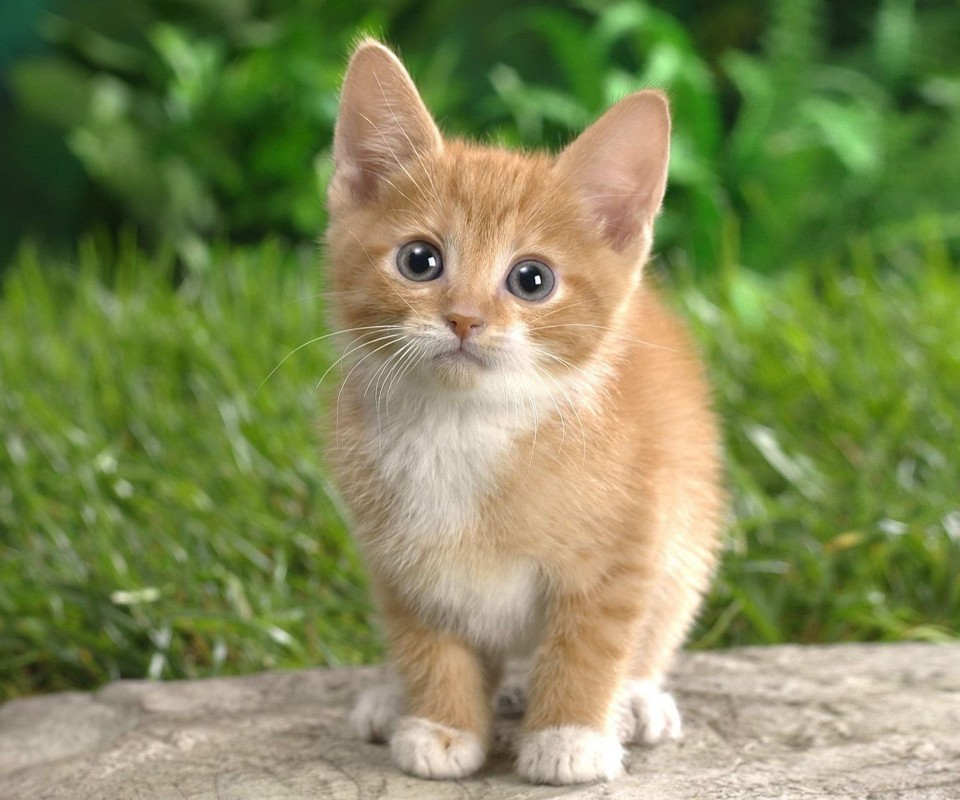
\includegraphics[width=0.3\textwidth]{images/kitten}
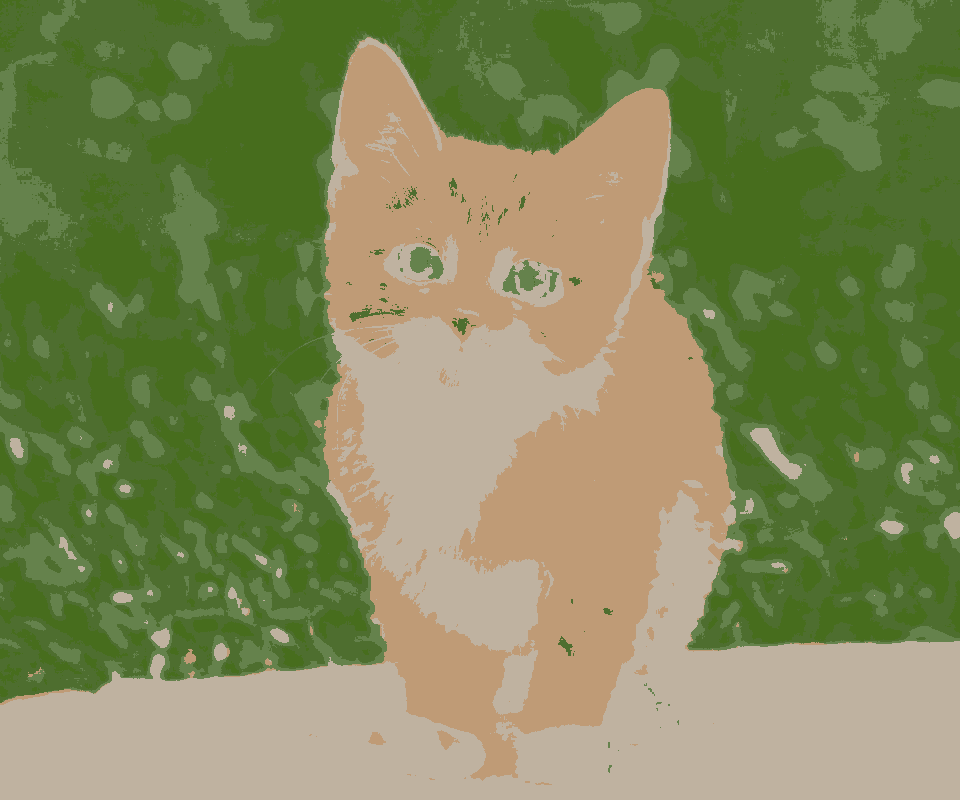
\includegraphics[width=0.3\textwidth]{images/hsv_5_kitten}
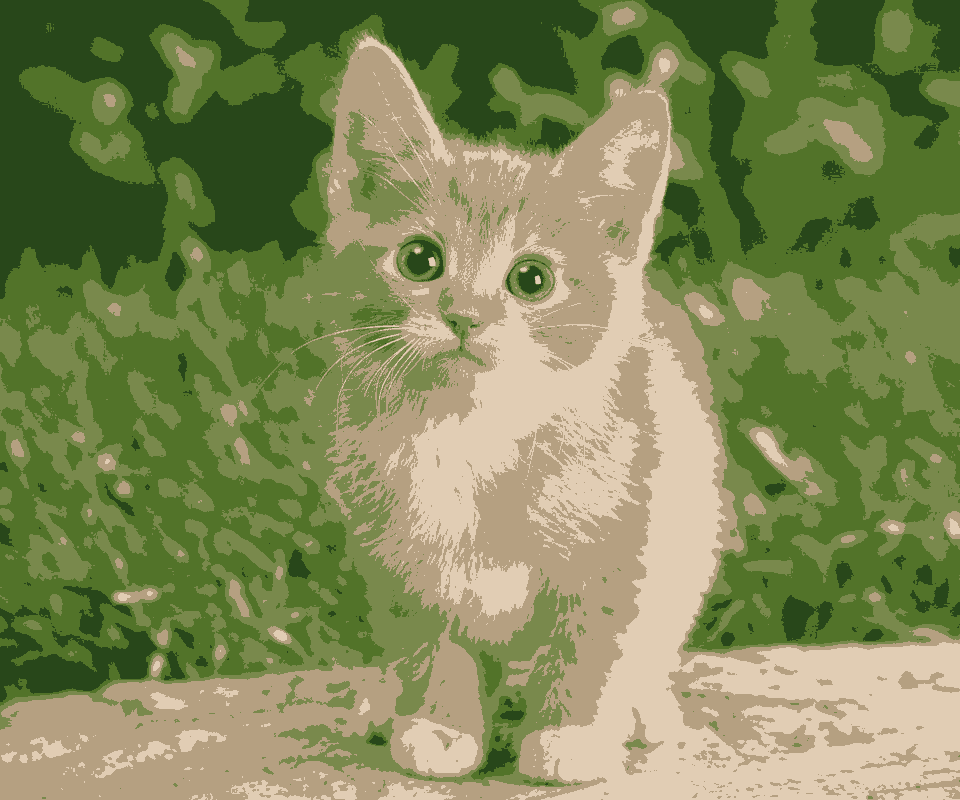
\includegraphics[width=0.3\textwidth]{images/rgb_5_kitten}
\caption{Kitten Original, HSV and RGB.}
\label{fig:kitten}
\end{center}
\end{figure}

\subsubsection{Sunset Tree k = 5}

\begin{figure}[ht]
\begin{center}
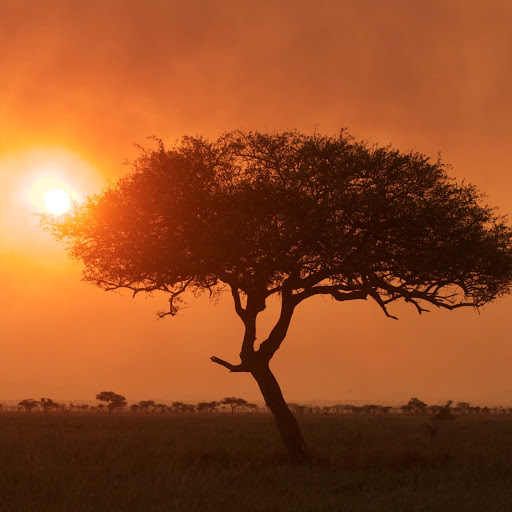
\includegraphics[width=0.3\textwidth]{images/sunset_tree}
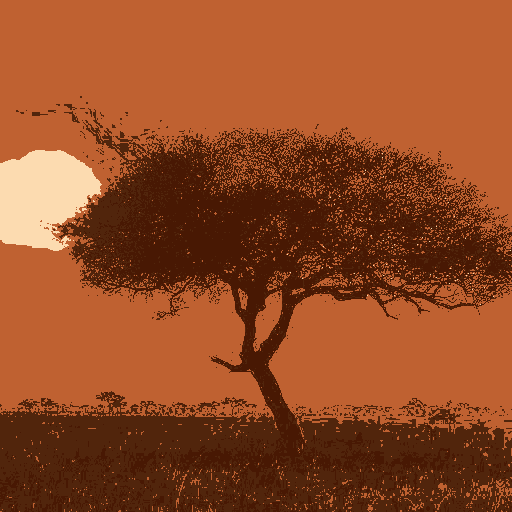
\includegraphics[width=0.3\textwidth]{images/hsv_5_sunset}
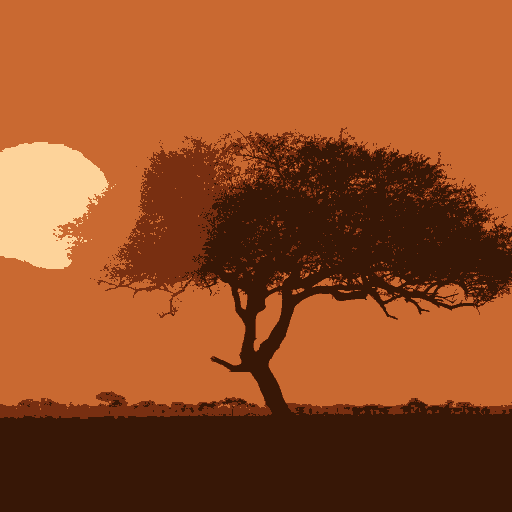
\includegraphics[width=0.3\textwidth]{images/rgb_5_sunset}
\caption{Sunset Tree Original, HSV and RGB.}
\label{fig:sunset}
\end{center}
\end{figure}

%---------------------------------------------------------------------------
% Strengths and Weaknesses
%---------------------------------------------------------------------------

\section{Strengths and Weaknesses}

Random Selection seems to perform worst than the others even though its
initialization takes the least amount of time. Overall the resulting images
typically miss colours that were in the original image, some colours like brown
seem turn into a darker colour like black. This is a result of how the selection
of clusters happens as if there is one missing colour from all the colours
selected as the starting clusters, then when the overall colours start to
average, they will move away from these colours and result in a different
result.\\
  
Random Clustering is by far superior than Random Selection as before
the k-means algorithm starts, the cluster colours are already averaged out over
the entire image. It allows for a more wide range of colours to be initialized
as the cluster colours. I have found with my testing that it helps with getting
out more colours from the image, which allows for when the segmentation to occur
that a lot of the colours appear in the final segmentation of the image.
k-means++ I have found is as good or better than Random Clustering. When
k-means++ is ran on a image it is good at getting more colours as the initial
clusters. I have found that when the colours are selected that there is more
smoothness around the edges of colours, such as when there are light spots or
shadows. Another thing I have noticed is that when there is a lot of colour in
the image white tends to be able to pop out and be properly segmented, whether
in the other two methods of initialization make the white blend in with other
colours.\\

In my implementation of RGB and HSV distance metric, RGB tends to perform better
than HSV, especially when there is a lot of colour in an image. The resulting
segmented images that RGB returns have a better image quality than HSV. However,
on images that are made up of predominantly one colour, HSV correctly segments
the image very well, compared to RGB.

%---------------------------------------------------------------------------
% End
%---------------------------------------------------------------------------

\end{document}
